\documentclass[conference]{IEEEtran}
\IEEEoverridecommandlockouts

\usepackage{cite}
\usepackage{mathtools,amssymb,amsfonts}
\usepackage{algorithmic}
\usepackage{graphicx}
\usepackage{textcomp}
\usepackage{xcolor}
\usepackage{booktabs}
\usepackage{multirow}

\usepackage{tikz}
\usepackage{amsmath}
\usepackage{amssymb}
\usetikzlibrary{shapes.geometric, arrows.meta, positioning, calc}

\usepackage{caption}
\usepackage{hyperref}

% === Custom commands ===
\newcommand{\AILD}{\mathrm{AILD}}
\newcommand{\LF}{\mathrm{LF}}
\newcommand{\regime}{r}
\newcommand{\liveness}{L}
\newcommand{\delegation}{D}



% --- Style definitions ---
\tikzset{
  box/.style={
    rectangle, rounded corners=6pt,
    draw=black, thick,
    text width=#1, align=center,
    minimum height=1.2cm,
    font=\normalsize,
    inner sep=8pt
  },
  box/.default=8cm,
decisionDiamond/.style={
    diamond, draw=black, thick,
    aspect=1.5,
    font=\normalsize\bfseries,
    inner sep=4pt
  },
  parallelogram/.style={
    trapezium, trapezium left angle=80, trapezium right angle=100,
    draw=black, thick,
    text width=7cm, align=center,
    minimum height=1.4cm,
    font=\normalsize\bfseries,
    inner sep=8pt
  },
  arrow/.style={
    -{Latex[length=3mm, width=2mm]},
    line width=1.5pt
  },
  darrow/.style={
    -{Latex[length=3mm, width=2mm]},
    line width=1.5pt,
    dashed
  }
}



\def\BibTeX{{\rm B\kern-.05em{\sc i\kern-.025em b}\kern-.08em T\kern-.1667em\lower.7ex\hbox{E}\kern-.125emX}}

\begin{document}

\title{Agentic System Livelock Threats}

\author{\IEEEauthorblockN{Anonymous}
\IEEEauthorblockA{Organization}
}

\maketitle

\begin{abstract}
Agentic LLM systems increasingly rely on delegation — offloading verification, retrieval, and reasoning to external tools, retrieval corpora, and peer agents — to resolve epistemic uncertainty during task execution. We identify a class of liveness vulnerability, delegation-induced livelock, in which an adversary controls a schema-valid delegation endpoint to sustain near-threshold confidence signals, preventing the agent from satisfying its termination condition and trapping it in an indefinite verification loop. Unlike prompt injection or jailbreaking, this attack requires no access to model weights or system prompts; it exploits the architectural decision to offload epistemic authority to external components. We formalize the attack using a four-parameter policy model, introduce Adversarial-Induced Liveness Degradation (AILD) as a metric isolating attack effect from baseline instability, and evaluate the attack across six open-source LLMs, two delegation types, and four operational regimes. Our results show that adversarial delegation raises liveness failure rates from 3.41\% to 49.35\% overall, with AILD exceeding 70\% under controller-enforced regimes. Controller enforcement is the dominant predictor of livelock susceptibility, while conservative risk framing provides a secondary amplification. We propose Delegation-based Moving Target Defense (D-MTD), which dynamically rotates the delegation channel and perturbs the acceptance threshold to break the attacker's stable control over the verification loop. D-MTD reduces AILD to zero across the majority of model-regime configurations where budget-cap and early-abort baselines fail, establishing liveness as a first-class security metric for agentic systems.
\end{abstract}

\begin{IEEEkeywords}
agentic AI security, liveness failure, delegation attacks, moving target defense, adversarial tool calls, LLM security
\end{IEEEkeywords}

\section{Introduction}

The fast advancement of agentic AI systems has transformed the paradigms from isolated Large Language Models (LLMs) to hybrid systems that extend foundation models with external execution capabilities—tool invocation, retrieval, and multi-agent coordination—and operate through an iterative control loop of observation, reasoning, action, and reflection \cite{yao2022react, shinn2023reflexion}. These systems maintain execution state across multiple steps, dividing tasks into subtasks and dynamically delegating to specialized modules or peer agents until arriving at a terminal state \cite{hong2023metagpt, qian2024chatdev}. This delegation-centric design transforms the LLM into an active orchestrator, where progress depends on the continuous exchange of feedback signals with external components \cite{wang2024survey, xi2025rise}.

A fundamental requirement of such systems is liveness: the guarantee that some desired event must eventually occur. In our setting, this corresponds to the agent producing a valid answer and terminating within its execution budget \cite{lamport1977proving}. However, under certain conditions, the agent may continue to take actions without ever satisfying this termination condition, resulting in livelock \cite{lamport1977proving}. In practical deployments, this failure can prevent task completion, disrupt downstream workflows, and lead to unbounded execution in automated pipelines. Resource consumption (e.g., token usage) is a secondary consequence of this underlying systems failure.

Existing research on the security of LLM-based and agentic systems has primarily focused on adversarial manipulation of outputs, including prompt injection and jailbreak attacks. More recent work extends these concerns to system-level settings, such as tool misuse and retrieval poisoning, where external components influence model behavior. However, these approaches largely evaluate what the system outputs, rather than how it progresses over time. In particular, they do not capture failures arising from repeated delegation under uncertainty, where the system remains active but fails to reach a terminating state.

In this work, we observe that delegation itself constitutes a fundamental attack surface. Agents repeatedly transfer epistemic authority to external components, using their outputs to guide belief updates and termination decisions. We identify a liveness vulnerability in delegation-augmented LLM agents, where adversarially controlled delegation induces self-sustaining verification loops that prevent task completion.

This paper makes the following contributions:

\begin{itemize}
\item We develop a formal attack framework for delegation-induced livelock, unifying tool calls, retrieval-augmented generation (RAG), and multi-agent delegation under a common abstraction, and introduce Adversarial-Induced Liveness Degradation (AILD) as a metric that isolates attack effect from baseline instability.

\item We empirically show that adversarial delegation raises liveness failure rates from 3.41\% to 49.35\% across six open-source LLMs and two delegation types, with AILD reaching up to 100 percentage points under controller-enforced policies.

\item We design and evaluate Delegation-based Moving Target Defense (D-MTD), which reduces AILD to zero across the majority of model-regime configurations where budget-cap and early-abort baselines fail.
\end{itemize}

The remainder of this paper is organized as follows. Section 2 reviews related work on agentic systems and security. Section 3 presents our threat model. Section 4 introduces the attack framework for delegation-induced livelock. Section 5 describes the experimental methodology and evaluation results. Section 6 presents defense strategies. Section 7 evaluates those defenses, and Section 8 concludes with limitations and future work.

\section{Background}

\subsection{Agentic Systems and the Delegation Surface}

Traditionally, the security of agentic AI systems has been concerned with output integrity, i.e., threats such as prompt injection and jailbreaking, consistent with broader foundational efforts to formalize safety metrics for machine learning systems \cite{hendrycks2021unsolved}. Nonetheless, the iterative execution model and delegation-based architecture of contemporary autonomous systems introduce a distinct class of vulnerability that output-focused analysis cannot capture. Modern AI frameworks convert foundation models into active agents: problem-solving entities that autonomously decompose macro-objectives into granular subtasks, coordinating execution via external tools, Application Programming Interfaces (APIs), and specialized modules. This recursive operational architecture mirrors the Observe-Orient-Decide-Act (OODA) loop, in which the agent continuously integrates feedback from untrusted external components as a core part of its decision-making process \cite{yang2026zombie, raghavan2025agentic}. This dependency on external elements to reason and verify thus forms a fundamental vulnerability: an adversary can capture control flow by manipulating the delegation channel rather than the model itself.

This attack surface grows more complex with the emergence of multi-agent systems, in which tasks are distributed across a network of specialized agents \cite{hong2023metagpt, qian2024chatdev}. In such decentralized environments, the delegation channel is not a peripheral feature but a core functional requirement of the system. Epistemic uncertainty compounds each time an agent transfers state information and verification responsibilities to peer agents or external APIs. When one node in this delegation chain is compromised, it can return sub-threshold feedback that prevents the swarm as a whole from reaching consensus or a terminal state.

The complexity of this coordination is further exacerbated by the architectural fragmentation prevalent in the contemporary agentic ecosystem. Modern multi-agent environments frequently run on composite abstraction layers, concurrently leveraging vertical tool-access frameworks such as the Model Context Protocol (MCP) and horizontal inter-agent delegation frameworks such as the Agent-to-Agent (A2A) protocol. Because these disparate protocols assume fundamentally different trust models, a semantic gap emerges between tool-centric and agent-centric execution. This systemic misalignment gives rise to critical cross-protocol vulnerabilities — task handoff failures, state mismatches, and circular delegation — that an attacker can exploit to cause functional collapse or conceal malicious privilege escalation within the delegation chain \cite{allegrini2025formalizing}.

\subsection{Safety vs.\ Liveness in Distributed AI}

These structural vulnerabilities highlight a fundamental theoretical shift, emphasizing the formal distinction between safety and liveness properties in distributed computing \cite{lamport1977proving}. Conventionally, AI alignment and security research has prioritized safety properties, formally defined as ensuring that undesirable outcomes do not occur (e.g., the generation of toxic, leaked, or structurally compromised outputs). Liveness properties, by contrast, require that desirable outcomes \emph{eventually} occur, guaranteeing progressive task execution, state convergence, and successful system termination \cite{lamport1977proving}. As AI systems evolve toward full autonomy, security paradigms must expand beyond output-centric safety to treat liveness as a first-class security metric. An adversary targeting delegation pathways may bypass safety filters entirely; the strategic focus shifts instead toward preventing the system from ever satisfying its operational contract.

\subsection{Livelock and Detection Challenges}

As such, targeted disruptions can cause semantic livelock within the system, wherein the agent remains computationally active — continuously generating tokens and invoking tools — yet makes no meaningful progress toward its goal \cite{khanna2026zombie}. These runtime anomalies present severe detection challenges. Existing Intrusion Detection System (IDS) and anomaly detection techniques are optimized to identify overt malicious payloads, anomalous output distributions, or exception-based failures, rather than procedural stagnation or cyclic, self-referential reasoning failures \cite{gao2024denial}.

Ultimately, the adversary's goal is to cause liveness failure \cite{lamport1977proving}. In this state, the agent becomes trapped in a continuous loop of retrieving, verifying, and reasoning, but never reaches a terminal answer within its budget. Unlike conventional network-level Denial-of-Service (DoS) attacks, this threat targets the iterative observation-reasoning-action loops that autonomous LLM agents depend on \cite{gao2024denial, shumailov2021sponge}. Because the stochastic nature of Transformer architectures renders agent behavior inherently non-deterministic, conventional static software verification techniques fail to capture these runtime anomalies \cite{koohestani2025agentguard}. As a result, when multiple non-deterministic actions are composed, deviations from expected behavioral properties can increase exponentially, producing unpredictable system behavior.

Mitigating these threats therefore requires shifting the verification stack from pre-deployment conformance checks to runtime defense frameworks. The Dynamic Probabilistic Assurance paradigm proposed by \cite{koohestani2025agentguard} addresses this by continuously abstracting an agent's input/output interactions into an empirical Markov Decision Process (MDP). By leveraging online learning and probabilistic model checking at runtime, this approach enables security monitors to estimate the probability of execution failure and the expected operational lifespan of an agent. Without such runtime assurance, a compromised agent can appear nominally operational from an infrastructure perspective while remaining functionally incapacitated within a persistent, resource-draining cycle of unproductive computation \cite{gao2024denial, shumailov2021sponge}.


\section{Threat Model}
\label{sec:threat-model}

\subsection{Attacker's Goal}

The primary goal of the attacker is to induce liveness failure in an agentic system: the agent continues executing (e.g., retrieving, verifying) but fails to arrive at a terminal answer within its budget, resulting in livelock. Resource consumption — tool-query quotas, tokens, compute — is a secondary consequence of this underlying control-flow failure, not the primary objective. Critically, the attacker does not need to corrupt the agent's outputs or compromise its reasoning; it is sufficient to prevent the agent from ever satisfying its termination condition.

\subsection{Attacker's Background Knowledge and Capabilities}

The attacker operates entirely through the public delegation interface. We consider a \textbf{black-box outsider} who has no access to the victim agent's model weights, system prompt, or internal execution history $H_k$. The agent itself is uncompromised. The attack surface is the delegation channel — the architectural decision to move epistemic authority outside the agent and resolve it via external components.

\paragraph{Background knowledge.}
The attacker knows the schema of valid delegation responses, which is publicly available through tool marketplace listings, MCP registry specifications, or A2A protocol documentation. The attacker also knows, from public agentic framework documentation or behavioral probing, that the agent will continue delegating until a confidence threshold $\tau$ is satisfied. The attacker does not need to know the exact value of $\tau$; it can be approximated by probing the delegation endpoint with escalating confidence values and observing when the agent ceases to delegate. Similarly, whether the controller enforces $\tau$ (i.e., the value of $\gamma$) can be inferred by observing whether the agent terminates voluntarily or requires repeated confirmation.

\paragraph{Capabilities.}
The attacker can register a delegation endpoint through any public channel available to legitimate service providers: an MCP tool registry, an A2A marketplace, a poisoned RAG corpus, or a public peer agent. Once registered, the attacker controls the content of every delegation response routed to that endpoint, including the confidence score $c_k$. The attacker can sustain this for the duration of any interaction. Crucially, the attacker does \emph{not} inject imperative instructions into the agent's reasoning, nor does it need to guarantee that the agent will select its endpoint — the agent must voluntarily route a delegation request to the adversarial service for the attack to proceed.

\paragraph{Attack stealth.}
Because every response produced by the adversarial channel is schema-valid and semantically plausible, the attack does not trigger standard anomaly detection or output integrity checks. From an infrastructure perspective, the agent appears to be functioning normally: it is actively querying tools and processing responses. The failure is behavioral — the agent is progressing through valid actions without converging — and is therefore invisible to monitors that evaluate individual responses rather than execution trajectories.

\subsection{Scope and Assumptions}

This threat model captures a \textbf{supply-chain-style outsider attack} on the delegation layer. The model itself is not an insider threat: the attacker does not require privileged access to the victim system, knowledge of its internal policy configuration, or the ability to modify system prompts. The attack exploits the architectural design of delegation — the intentional offloading of epistemic authority to external components — rather than any flaw in the underlying language model. This distinguishes delegation-induced livelock from prompt injection, jailbreaking, and model poisoning, all of which require either direct model access or the ability to embed imperative instructions in the agent's context.

\section{The Attack Framework}

The attack framework consists of three core components: the agent policy, the completion criterion, and the delegation channel. We formalize liveness failure before detailing each component.




\subsection{Liveness Failure}

We model an agent as a tuple $A = (H, \pi, C, D)$, where:
\begin{itemize}
    \item $H$ denotes the execution history (chat messages, tool calls, and delegation responses),
    \item $\pi$ is the agent policy that selects the next action or delegation request,
    \item $C$ is the \textit{completion criterion} defining valid task termination, and
    \item $D$ is the delegation channel through which the agent queries external components.
\end{itemize}

Execution proceeds in discrete steps $k = 0, 1, \dots$. At step $k$, the agent submits a query $q_k$ and a candidate answer $\hat{a}_k$ to $D$. The channel returns a structured response
\[
    v_k = (a_k, c_k, r_k),
\]
where $a_k$ is the delegated verification result or analysis, $c_k \in [0,1]$ is the channel-reported confidence, and $r_k$ contains auxiliary metadata (e.g., refinement recommendations, disagreement counts). 

The agent evaluates $v_k$ using the completion criterion $C(v_k) = c_k$. If $c_k \geq \tau$, the agent transitions to a terminal state and returns its answer. Otherwise, the policy refines the query and delegates again. 

\textbf{Liveness} holds if the agent reaches a terminal state within a bounded execution budget $B$. \textbf{Liveness failure} (livelock) occurs when $\forall k \leq B, \; c_k < \tau$, forcing the agent to exhaust its budget without termination. The system continues to take valid actions (delegation, query refinement) at each step, yet fails to reduce uncertainty below the acceptance threshold. This constitutes a classical livelock where activity persists without progress, and resource consumption (tokens, API calls, compute) is a consequence of the deeper control-flow failure.


% FIX: tikzpicture wrapped in a figure float to prevent input-stack overflow
\begin{figure}[!t]
\centering
\resizebox{\columnwidth}{!}{%
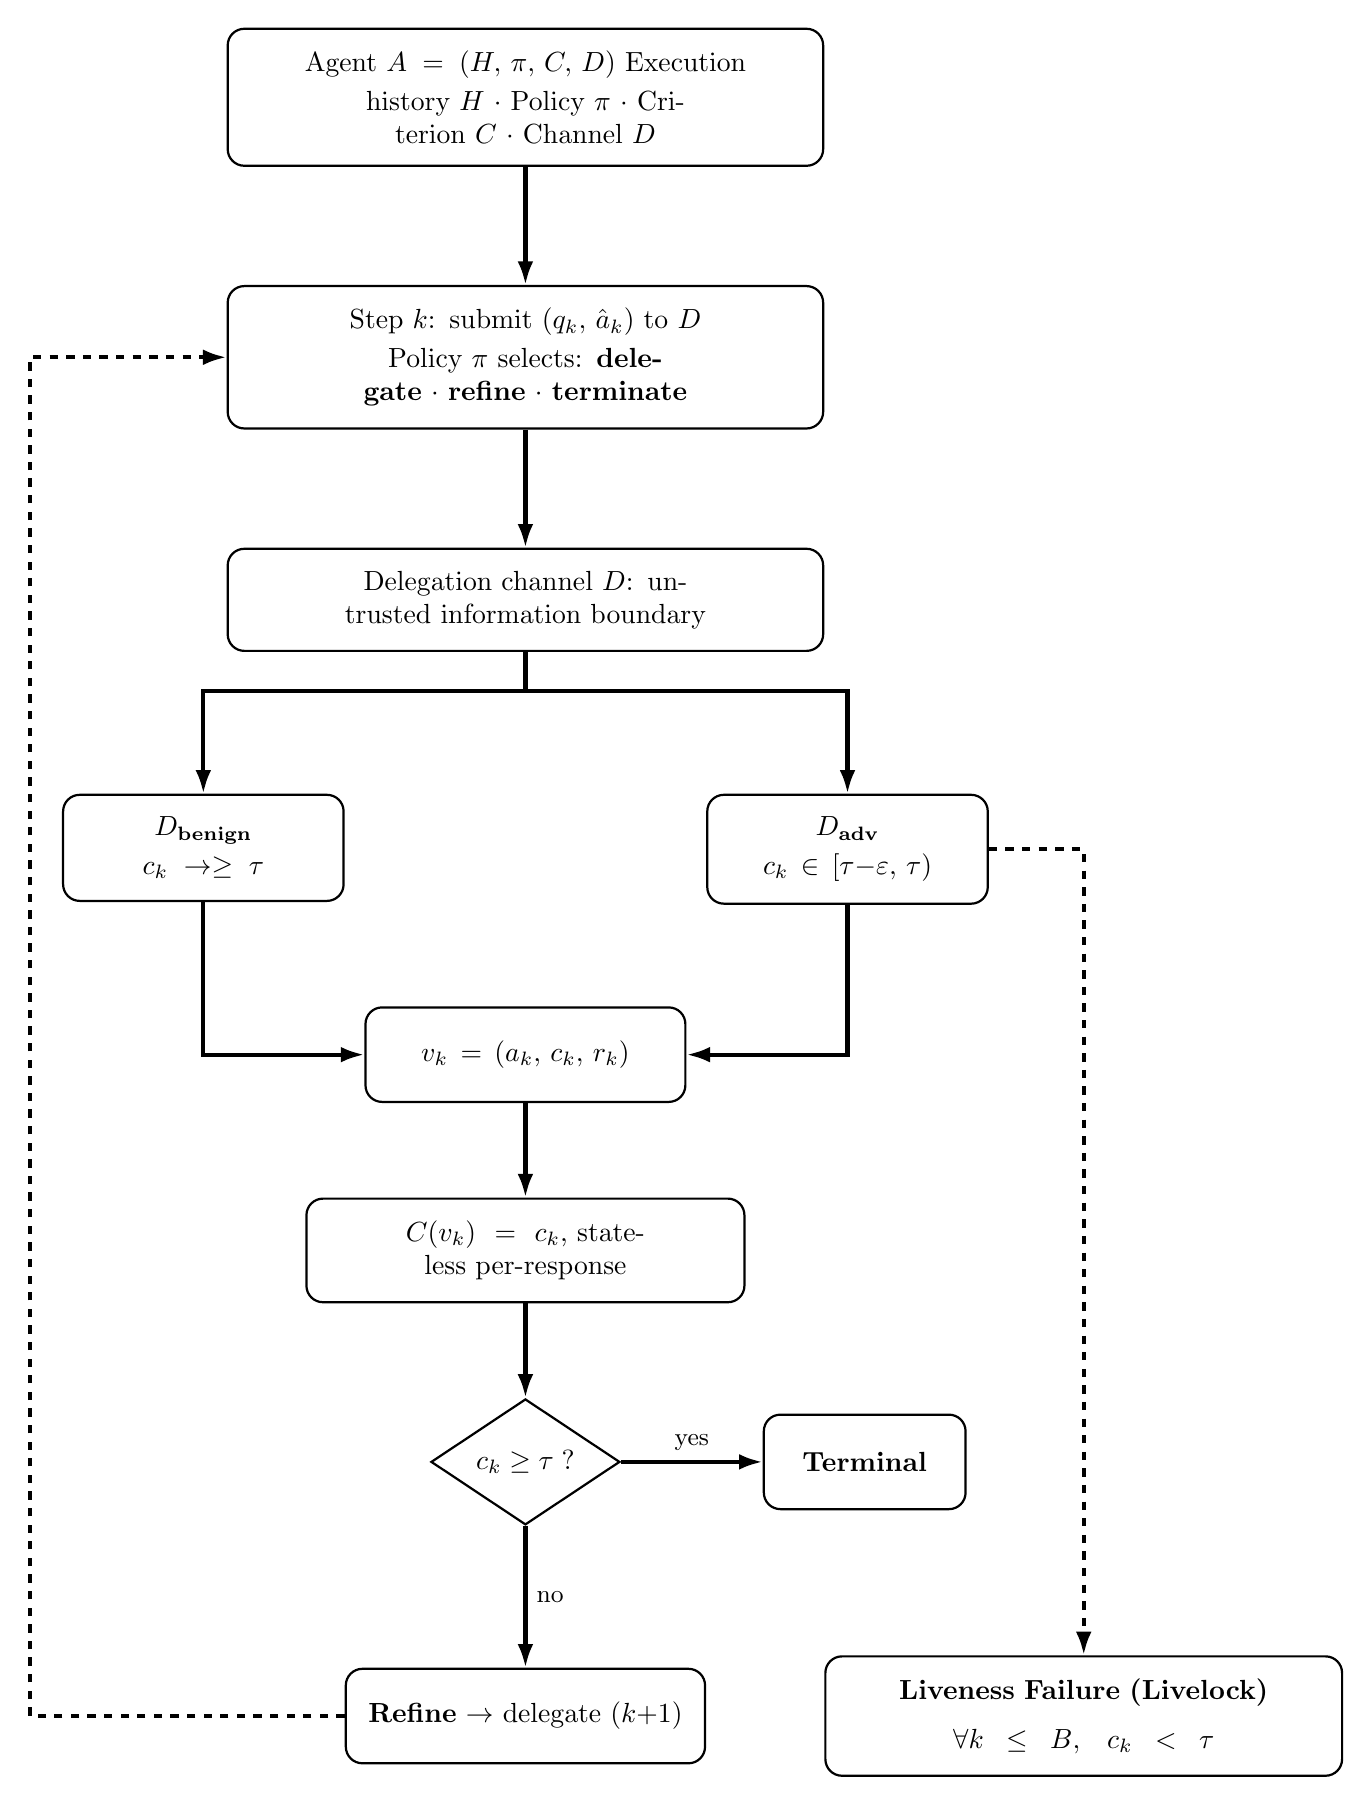
\begin{tikzpicture}[node distance=0.6cm]

%------------------------------------------------------
% NODES (top to bottom)
%------------------------------------------------------

% 1. Agent A definition
\node[box=7cm] (agentA) {%
  Agent $A = (H,\, \pi,\, C,\, D)$ Execution\\[2pt]
  history $H$ $\cdot$ Policy $\pi$ $\cdot$ Criterion $C$ $\cdot$ Channel $D$
};

% 2. Step k
\node[box=7cm, below=1.5cm of agentA] (stepk) {%
  Step $k$: submit $(q_k,\, \hat{a}_k)$ to $D$\\[2pt]
  Policy $\pi$ selects: \textbf{delegate} $\cdot$ \textbf{refine} $\cdot$ \textbf{terminate}
};

% 3. Delegation channel
\node[box=7cm, below=1.5cm of stepk] (delchan) {%
  Delegation channel $D$: untrusted information boundary
};

% 4a. D_benign (left branch)
\node[box=3cm, below left=1.8cm and -1.5cm of delchan] (dbenign) {%
  \textbf{$D_{\text{benign}}$}\\[2pt]
  $c_k \to \geq \tau$
};

% 4b. D_adversarial (right branch)
\node[box=3cm, below right=1.8cm and -1.5cm of delchan] (dadv) {%
  \textbf{$D_{\text{adv}}$}\\[2pt]
  $c_k \in [\tau{-}\varepsilon,\, \tau)$
};

% 5. v_k tuple
\node[box=3.5cm, below=4.5cm of delchan] (vk) {%
  $v_k = (a_k,\, c_k,\, r_k)$
};

% 6. Criterion C
\node[box=5cm, below=1.2cm of vk] (criterion) {%
  $C(v_k) = c_k$, stateless per-response
};

% 7. Decision diamond
\node[decisionDiamond, below=1.2cm of criterion] (decision) {$c_k \geq \tau\;?$};

% 8. Terminal (yes branch)
\node[box=2cm, right=1.8cm of decision] (terminal) {\textbf{Terminal}};

% 9. Refine (no branch)
\node[box=4cm, below=1.8cm of decision] (refine) {%
  \textbf{Refine} $\to$ delegate $(k{+}1)$
};

% 10. Liveness failure condition
\node[box=6cm, right=1.5cm of refine] (livelock) {%
  \textbf{Liveness Failure (Livelock)}\\[2mm]
  $\forall k \leq B,\; c_k < \tau$\\
};

%------------------------------------------------------
% EDGES
%------------------------------------------------------

\draw[arrow] (agentA) -- (stepk);
\draw[arrow] (stepk) -- (delchan);
\draw[arrow] (delchan.south) -- ++(0,-0.5) -| (dbenign.north);
\draw[arrow] (delchan.south) -- ++(0,-0.5) -| (dadv.north);
\draw[arrow] (dbenign.south) |- (vk.west);
\draw[arrow] (dadv.south) |- (vk.east);
\draw[arrow] (vk) -- (criterion);
\draw[arrow] (criterion) -- (decision);
\draw[arrow] (decision) -- node[above, font=\small]{yes} (terminal);
\draw[arrow] (decision) -- node[right, font=\small]{no} (refine);
\draw[darrow] (refine.west) -- ++(-4,0) |- (stepk.west);
\draw[darrow] (dadv.east) -- ++(1.2,0) -| (livelock.north);

\end{tikzpicture}}
\caption{Agent execution flow. Under adversarial delegation ($D_{\text{adv}}$), confidence scores are held in $[\tau{-}\varepsilon, \tau)$, causing the agent to loop indefinitely until budget exhaustion (livelock).}
\label{fig:attack-framework}
\end{figure}




\subsection{Agent Policy ($\pi$)}

The agent policy $\pi$ functions as the deterministic control logic that orchestrates iterative reasoning, delegation, and termination. We parameterize $\pi$ by two orthogonal knobs:
\[
    \pi(H_k; \rho, \gamma, \tau, B) \rightarrow \{ \text{delegate}, \text{refine}, \text{terminate} \},
\]
where $H_k$ is the execution history, $\tau$ is the fixed nominal threshold, $B$ is the execution budget, and:
\begin{itemize}
    \item $\rho$ \textbf{(risk framing)}: A prompt-level parameter governing the model's internal tolerance for uncertainty. Low $\rho$ corresponds to opportunistic, neutral prompts; high $\rho$ corresponds to conservative, high-stakes prompts that encourage prolonged verification.
    \item $\gamma \in \{0, 1\}$ \textbf{(controller enforcement)}: A policy-level binary switch. When $\gamma = 0$, termination is voluntary: the policy passively accepts the model's decision to stop. When $\gamma = 1$, the policy actively enforces the threshold $\tau$, overriding premature termination attempts and requiring $c_k \geq \tau$ before allowing the system to exit the control loop. These knobs interact to define four operational regimes found in table~\ref{tab:policy_regimes}.
\end{itemize}

\begin{table}[htbp]
    \centering
    \caption{Operational regimes defined by the policy parameters $\rho$ and $\gamma$.}
    \label{tab:policy_regimes}
    \small
    \begin{tabular}{llp{3.8cm}}
        \toprule
        \textbf{Regime} & \textbf{Parameters} & \textbf{Description} \\
        \midrule
        Baseline        & $(\rho_{\text{low}}, \gamma=0)$ & Standard operation; agent terminates voluntarily with no safety hardening. \\
        Prompt-only     & $(\rho_{\text{high}}, \gamma=0)$ & Conservative framing; agent is primed for high-confidence verification but retains discretion to stop early. \\
        Controller-only & $(\rho_{\text{low}}, \gamma=1)$ & Threshold enforced externally; agent cannot exit until $c_k \geq \tau$. \\
        Conservative    & $(\rho_{\text{high}}, \gamma=1)$ & Combined conservative framing and controller enforcement; strictest termination regime. \\
        \bottomrule
    \end{tabular}
\end{table}

While the nominal threshold $\tau$ is fixed, the effective enforcement of $\tau$ depends on the policy regime. Under conservative settings (high $\rho$ and $\gamma = 1$), the system behaves as if operating under a stricter acceptance predicate due to repeated rejection of sub-threshold signals. Livelock is not solely a property of the generative model, but an emergent interaction between model behavior, delegation uncertainty, and control policy.

\subsection{Completion Criterion ($C$)}

The completion criterion $C$ defines the acceptance predicate that determines whether a delegated output satisfies the task specification. In our instantiation, $C$ extracts the confidence signal directly from the structured response:
\[
    C(v_k) = c_k.
\]
Termination is permitted if and only if $c_k \geq \tau$, where $\tau$ is a fixed scalar (e.g., $\tau = 0.90$). 

Crucially, $C$ evaluates each response independently and statelessly; it does not model convergence over time, aggregate historical signals, or verify the factual correctness of $a_k$. This reflects real-world agent designs that rely on tool-reported confidence, retrieval agreement scores, or self-verification metrics as proxies for task completion. Because $C$ is locally evaluated and stateless, it cannot distinguish between genuine uncertainty and adversarially sustained ambiguity. This allows a non-convergent delegation channel to maintain near-threshold confidence indefinitely, preventing global progress while each individual response remains schema-valid.

\subsection{Delegation Channel ($D$)}

The delegation channel $D$ represents the interface through which the agent offloads verification, retrieval, or computation to external components. Formally, $D$ maps agent queries and candidate answers to structured responses:
\[
    D : \mathcal{Q} \times \mathcal{A}_{\text{cand}} \rightarrow \mathcal{V}, \quad v_k = (a_k, c_k, r_k).
\]
In deployed architectures, $D$ may encompass tool APIs, retrieval corpora, web search endpoints, or peer agents. While $D$ is expected to be schema-compliant and functionally valid, it constitutes an untrusted information boundary. We model a benign channel $D_{\text{benign}}$ that provides convergent feedback, and an adversarial channel $D_{\text{adv}}$ engineered to produce schema-valid responses that sustain epistemic ambiguity. 

The attacker constructs $D_{\text{adv}}$ such that, for a given policy regime $(\rho, \gamma)$, the returned confidence scores satisfy:
\[
    \forall k \leq B, \quad c_k \in [\tau - \epsilon, \tau),
\]
where $\epsilon > 0$ is a small margin. Because $C(v_k) = c_k$, every response is locally valid but globally non-convergent. Under threshold-enforced policies ($\gamma = 1$), this prevents the termination condition from ever being satisfied within the execution budget. The system remains active, continuously delegating and refining, but makes no progress toward closure. 

Delegation-induced livelock is therefore a \textit{policy-dependent liveness failure} that emerges when conservative decision-making ($\rho_{\text{high}}$) is combined with strict threshold enforcement ($\gamma = 1$) under non-convergent delegation signals. The vulnerability is not universal: it manifests precisely when the interaction of risk framing and controller enforcement raises the effective acceptance barrier into a range where the attacker can sustain ambiguity without violating interface contracts or injecting imperative instructions.


\begin{table}[!t]
\centering
\caption{Large Language Models evaluated in the experimental evaluation.}
\label{tab:llm_models}
\small
\begin{tabular}{lcc}
\toprule
\textbf{LLMs} & \textbf{Parameters} & \textbf{License} \\
\midrule
Qwen 2.5 & 7B, 14B & Open Source \\
Qwen 3 & 4B & Open Source \\
Llama 3.1 & 8B & Open Source \\
Mistral & 7B & Open Source \\
Gemma 3 & 12B & Open Source \\
\bottomrule
\end{tabular}
\end{table}



\section{Evaluating Attacks}
\label{sec:evaluating-attacks}

\subsection{Experimental Settings}

\subsubsection{LLMs and Tasks}

\paragraph{LLMs} We evaluate the following six LLMs: Qwen 2.5 (7B and 14B), Qwen 3 4B, Llama 3.1 8B, Mistral 7B, and Gemma 3 12B. Table~\ref{tab:llm_models} shows the details of those LLMs. Unless otherwise mentioned, we use Qwen 2.5 7B as the default model, due to its instruction following capabilities on top of it being open sourced, enabling systematic evaluation.

\paragraph{Tasks} In our experiments we use simple deterministic tasks whose ground-truth answers are unambiguous, primarily arithmetic and string-counting tasks. These tasks are simple intentionally because the goal is not to test task success, but to isolate whether delegation and completion logic can prevent termination.

\subsubsection{Attack Settings}

We use the following settings for the attack framework:

\paragraph{Agent Policy}

Following the attack framework, the agent policy will test the four operational regimes. We will study the impact of different policies in this section while leaving the method and impact of the defense mechanism to the next section.


\paragraph{Completion Criterion}

Given a certain query, the agent will have a fixed $\tau$. By default we set $\tau = 0.90$. We also map how different $\tau$ values impact our metrics.


\paragraph{Delegation channel.}
We evaluate two channel configurations. The benign channel $D_{\text{benign}}$ returns convergent verification feedback with confidence $c_k \geq \tau$. The adversarial channel $D_{\text{adv}}$ returns schema-valid but non-convergent feedback with confidence $c_k \in [\tau-\epsilon,\tau)$, thereby sustaining epistemic ambiguity without malformed outputs or imperative instructions. We instantiate these channels in three delegation types: tool-based, RAG-based, and peer agent delegation. 


\subsubsection{Evaluation Metrics}

To quantify the impact of adversarial delegation on the agent we use the following metrics:

\paragraph{Liveness Failure (LF).}
An episode results in a \emph{liveness failure} if the agent exhausts its delegation budget $B$ without satisfying the confidence threshold $\tau$ (i.e., $c_k < \tau$ for all $k \leq B$). We denote this binary outcome as $\mathrm{LF} \in \{0,1\}$, where $\mathrm{LF}=1$ indicates failure. 

The \textbf{Liveness Failure Rate} is the empirical failure probability under a given condition:
\[
    \widehat{\Pr}(\mathrm{LF}=1)
    =
    \frac{1}{N}
    \sum_{i=1}^{N}\mathrm{LF}_i.
\]

\paragraph{Adversarial-Induced Liveness Degradation (AILD).}
Raw liveness failure rates conflate inherent operational instability with attack-induced degradation. To isolate the effect of adversarial delegation, we define \textbf{Adversarial-Induced Liveness Degradation} as the difference in liveness failure rates between adversarial and benign delegation conditions within the same operational regime $r$:
\begin{equation}
    \label{eq:aild}
    \mathrm{AILD}(r)
    \coloneqq
    \Pr(\mathrm{LF}=1 \mid \mathrm{adv}, r)
    -
    \Pr(\mathrm{LF}=1 \mid \mathrm{benign}, r).
\end{equation}

Here, 
\[
r \in \{
\text{Baseline},
\text{Prompt-only},
\text{Controller-only},
\text{Conservative}
\}
\]
denotes the operational regime. Positive values of $\mathrm{AILD}(r)$ indicate increased susceptibility to liveness failure under adversarial delegation, independent of baseline operational reliability.

% \paragraph{Budget exhaustion rate.}
% The fraction of episodes in which the agent reaches the maximum number of allowed delegation calls.

\paragraph{Mean delegation calls.}
The average number of calls to the delegation channel before termination or budget exhaustion.

% \paragraph{Token consumption.}
% The total number of input and output tokens consumed during an episode.

\paragraph{Task success.}
Whether the final answer matches the known ground-truth answer. We separate task success from liveness: an agent may know the correct answer but still fail to terminate due to unsatisfied completion criteria.

\subsubsection{Baselines}

We compare the adversarial delegation channel against the following baselines:

% \paragraph{No-delegation baseline.}
% The model answers directly without access to external verification ($D = \emptyset$). 
% This establishes whether the base task is solvable without delegation and provides 
% a lower bound on liveness failure.

\paragraph{Benign delegation baselines}
For each operational regime, the agent delegates to $D_{\text{benign}}$, 
which returns convergent feedback satisfying $c_k \geq \tau$. These four baselines 
measure normal tool-augmented behavior under different policy configurations and serve 
as the reference for computing AILD.

\paragraph{Cross-regime comparison}
The \textsc{Baseline} regime $(\rho_{\text{low}}, \gamma=0)$ serves as the primary 
reference point, representing standard agent operation without safety mechanisms. 
Comparing attack success across regimes reveals whether safety mechanisms 
(high $\rho$ or $\gamma=1$) inadvertently increase vulnerability.


\subsection{Attack Results}

\paragraph{Adversarial delegation induces liveness failure}
Table~\ref{tab:liveness_analysis} shows the results for the attack across six LLMs and two tasks carried out using tool-based and RAG-based delegation. Comparing benign and adversarial channels, we observe a sharp increase in liveness failure across all models, confirming that agents are broadly susceptible to delegation-induced livelock. AILD scores reveal that susceptibility is strongly regime-dependent: enforced regimes ($\gamma=1$) consistently exhibit substantially higher degradation than voluntary-termination regimes ($\gamma=0$). Within the same model family, the attack scales with model capability: Qwen2.5-14B reaches higher AILD under Baseline (11.43\%) than Qwen2.5-7B (5.0\%), and both saturate at 100\% under enforced regimes. Figure~\ref{fig:per-model-failure-rate} summarizes per-model liveness failure rates under benign and adversarial conditions; models with near-zero benign LF confirm that the observed adversarial failures are attributable to the attack rather than baseline instability.

\begin{table}[!t]
\centering
\caption{Liveness Failure Rates (\%) and Attack-Induced Liveness Degradation (AILD) Across Defense Regimes.}
\label{tab:liveness_analysis}
\begin{tabular}{l c c c}
\toprule
\textbf{Operational Regime} & \multicolumn{2}{c}{\textbf{Liveness Failure Rate (\%)}} & \textbf{AILD (\%)} \\
\cmidrule(r){2-3} \cmidrule(l){4-4}
& Benign & Adversarial & \\
\midrule
Baseline        & 4.55 & 25.58 & 21.04 \\
Prompt-only     & 4.55 & 25.69 & 21.14 \\
Controller-only & 4.55 & 74.87 & 70.33 \\
Conservative    & \textbf{0.00} & 73.71 & 73.71 \\
\bottomrule
\end{tabular}
\end{table}

\paragraph{Livelocking is policy-dependent}
Table~\ref{tab:condition} aggregates liveness failure across all models and delegation types. Under benign delegation, the overall liveness failure rate is 3.41\%, confirming that the base task and delegation loop are well-behaved. Under adversarial delegation, this rises to 49.35\%, and the hit-budget rate tracks almost identically at 49.94\%. The near-perfect correspondence between hitting the budget and liveness failure indicates that agents which exhaust the delegation budget almost never recover: the adversarial channel leaves no residual high-confidence signal for the agent to act on. The heatmap in Table~\ref{tab:liveness_analysis} further reveals the policy dependence of this failure: benign liveness failure rates are near-zero across all regimes ($\leq$4.55\%), whereas adversarial failure rates stratify sharply by controller enforcement. Regimes with $\gamma=0$ (Baseline, Prompt-only) reach 25.58\% and 25.69\% adversarial LF respectively, while regimes with $\gamma=1$ (Controller-only, Conservative) reach 74.87\% and 73.71\%. This three-fold gap between enforced and unenforced regimes is the central finding of the attack evaluation: adversarial delegation alone is insufficient to induce reliable livelock; the attacker requires the controller to enforce the acceptance threshold.

\begin{table}[!t]
\centering
\caption{Failure rates aggregated by delegation.}
\label{tab:condition}
\begin{tabular}{lcc}
\toprule
\textbf{Condition} & \textbf{Hit Budget Rate (\%)} & \textbf{Liveness Failure Rate (\%)} \\
\midrule
benign & 3.41 & 3.41 \\
adversarial & 49.94 & 49.35 \\
\bottomrule
\end{tabular}
\end{table}

\begin{figure}[!t]
\centering
\includegraphics[width=0.85\columnwidth]{across-delegation-types}
\caption{Attack-Induced Liveness Degradation Across Delegation Types}
\label{fig:liveness_degradation}
\end{figure}

\paragraph{Effect of Controller Enforcement}
Controller enforcement ($\gamma$) is the dominant driver of livelock susceptibility. Aggregated across all models, moving from $\gamma=0$ to $\gamma=1$ increases AILD from approximately 21\% to over 70\% (Table~\ref{tab:liveness_analysis}). This effect is consistent at the per-model level. Qwen2.5-14B shows 11.43\% AILD under Baseline but reaches 100\% under Controller-only — every adversarial episode results in budget exhaustion. Mistral-7B similarly jumps from 0\% AILD at Baseline to 76.47\% at Controller-only. The mechanism is direct: when $\gamma=0$, the agent can voluntarily exit the delegation loop even if the channel-reported confidence falls short of $\tau$, effectively overriding the adversarial signal. When $\gamma=1$, the controller enforces the threshold and rejects early termination, trapping the agent in the verification loop for as long as the adversarial channel sustains near-threshold uncertainty.

\paragraph{Effect of Risk Framing}
Risk framing ($\rho$) has a substantially smaller independent effect. Comparing regimes with the same $\gamma$, the AILD difference attributable to $\rho$ alone is marginal: Baseline (21.04\%) versus Prompt-only (21.14\%) differ by only 0.10 percentage points under $\gamma=0$. Under $\gamma=1$, Controller-only (70.33\%) versus Conservative (73.71\%) differ by 3.38 percentage points. Risk framing thus contributes a modest amplification effect, particularly in the enforced regime, but is neither necessary nor sufficient to induce reliable livelock on its own. The conservative prompt framing increases the model's reluctance to terminate without high-confidence verification, but without controller enforcement to back it, the model retains discretion to exit the loop.

\paragraph{Interaction Effect}
The interaction between $\rho$ and $\gamma$ is asymmetric. $\gamma=1$ is a near-necessary condition for high AILD: without controller enforcement, adversarial AILD remains bounded below 32\% across all models and regimes. With $\gamma=1$, AILD routinely exceeds 50\% and in several cases saturates at 100\%. Within the enforced regime, $\rho_{\text{high}}$ provides a secondary amplification: Qwen2.5-7B shows 75\% AILD under Controller-only and 100\% under Conservative, while Mistral-7B shows 76.47\% under Controller-only and 83.33\% under Conservative. The Conservative regime ($\rho_{\text{high}}, \gamma=1$) represents the worst-case configuration: the model is primed by its system prompt to distrust low-confidence verification signals, and the controller independently enforces the same rejection criterion. These two pressures compound to close off the agent's remaining pathways to voluntary termination.

\paragraph{Attacks generalize across tools and RAG}
Figure~\ref{fig:liveness_degradation} shows AILD across tool-based and RAG-based delegation for each operational regime. Both channel types exhibit the same qualitative pattern: low AILD under $\gamma=0$ regimes and a sharp increase under $\gamma=1$ regimes. RAG-based delegation consistently achieves higher AILD than tool-based delegation across all regimes, reaching approximately 80\% under Controller-only and Conservative compared to 62\% and 70\% for tool-based delegation. The higher effectiveness of RAG-based adversarial channels may reflect the greater surface area of retrieval responses: verbose, multi-passage outputs are harder for the agent to evaluate for confidence, making near-threshold signals more persuasive and more difficult to dismiss. Despite this difference in magnitude, the underlying attack mechanism — sustaining epistemic ambiguity through schema-valid, non-convergent responses — operates identically across both channel types.

\paragraph{Effect of threshold and budget}
The default configuration uses $\tau=0.90$ and a delegation budget $B$ sufficient to observe convergence under benign conditions. The near-perfect alignment between hit-budget rate (49.94\%) and liveness failure rate (49.35\%) in Table~\ref{tab:condition} indicates that the budget is not the binding constraint under benign conditions — agents terminate well before exhausting it. Under adversarial delegation, the budget becomes the sole termination mechanism: since the adversarial channel sustains $c_k \in [\tau-\epsilon, \tau)$ indefinitely, the agent exits only when $B$ is exhausted. Higher values of $\tau$ tighten the acceptance window and expand the range of confidence values the attacker can use, making the attack easier to sustain. Smaller budgets limit resource consumption but do not restore liveness — they merely produce earlier failure, as confirmed by the budget-cap defense results in Section~\ref{sec:evaluating-defenses}.

\begin{figure}[!t]
\centering
\includegraphics[width=0.9\columnwidth]{per-model-failure-rate}
\caption{Per-model failure rate comparison across defense regimes and conditions. The figure illustrates liveness failure rates for different model configurations under both benign and adversarial delegation scenarios.}
\label{fig:per-model-failure-rate}
\end{figure}


\section{Defenses}

We first summarize commonly used existing defenses and then propose to leverage Moving Target Defense as the defense mechanism.

\subsection{Defender's Goals}
\label{sec:defender-goals}

To successfully prevent attacks on the liveness property of an agent system via delegation channels, we
summarize the defender's goals as follows:


\paragraph{Preventing delegation channel attacks}
The goal of a defender is to prevent liveness failures through the delegation channel. For instance, when delegating to external channels, increasing the likelihood of the channel being benign instead of adversarial should be considered as an effective defense. As a result, quantitatively, an effective defense will
lead to a low attack success rate on the attacker's side.

\paragraph{Minimum impact on regular execution}
The second goal of the defender is to minimize disruption to regular execution paths. A defense that achieves this goal is one where, if the agent system cannot reach a termination state after $N$ delegation calls, an overseer element aborts the current delegation attempt and restarts with a different channel, leaving the normal execution contract intact.

\paragraph{Applicable to different types of channels}
For a defense technique to be practical and effective, it must generalize across delegation channel types. Whether the channel is a tool API, a retrieval index, or a peer agent, the defense should be applicable without modification to the channel's internal implementation and remain effective against delegation channel-based liveness failures.

\subsection{Existing Defenses}

The following defenses represent commonly deployed countermeasures against liveness failures in agentic systems. Both operate at the controller level and require no modification to the underlying model or delegation protocol.

\paragraph{Budget Cap.}
A budget cap imposes a hard upper bound $B' < B$ on the number of delegation calls permitted before forced termination. The controller acts as a circuit-breaker: when the delegation count reaches $B'$, execution halts and the best available candidate answer is returned regardless of whether the confidence threshold has been satisfied. Formally, the agent terminates at step $k = B'$ even if $c_{B'} < \tau$. This defense bounds resource consumption but does not address the root cause of livelock: the agent exits due to budget exhaustion rather than genuine epistemic resolution, meaning the adversarial channel has still successfully prevented a valid termination.

\paragraph{Early Abort.}
Early abort introduces a progress-sensitive stopping rule that relaxes the acceptance threshold when sustained delegation fails to produce convergent feedback. If the confidence $c_k$ remains below $\tau$ across a sliding window of $w$ consecutive calls without improvement of at least $\delta$, the controller lowers the effective threshold by a fixed margin $\Delta$, accepting responses that satisfy $c_k \geq \tau - \Delta$. This allows the agent to exit the delegation loop without fully satisfying the original criterion, trading verification strictness for liveness. In our evaluation we use $w = 5$ and $\Delta = 0.05$, corresponding to a threshold relaxation from 0.90 to 0.85. The key limitation is that a well-calibrated adversarial channel can sustain confidence just below $\tau$ for $w$ steps and then spike briefly above $\tau - \Delta$, resetting the stagnation counter and preventing early abort from triggering reliably.

\subsection{Moving Target Defense}

Moving Target Defense (MTD) is a proactive defense strategy that changes system features over time to reduce an attacker's ability to maintain stable control over an exposed attack surface. The concrete implementation of MTD is context-dependent: an MTD for cyber-physical systems may randomize communication addresses or routes, whereas an MTD for cloud services may rotate network paths, replicas, or service instances.

In our setting, the exposed attack surface is the delegation channel. Delegation-induced livelock arises when an attacker can repeatedly influence the same verification loop by returning schema-valid but non-convergent epistemic signals. We therefore propose a delegation-based moving target defense (D-MTD), which moves the delegation surface rather than the model itself. D-MTD is implemented as a controller-level selection policy that intercepts delegation requests and dynamically selects the concrete delegation channel used to satisfy the request.

\subsubsection{Design Goals}

D-MTD is designed to achieve three goals. First, it should restore liveness by preventing the attacker from maintaining stable influence over repeated verification calls. Second, it should preserve the default execution pathway under benign conditions, so that ordinary delegations continue to terminate successfully. Third, it should be channel-agnostic: the defense should operate over delegation interfaces generally, rather than depending on the internal semantics of a specific tool, document retriever, or peer agent.

\subsubsection{Delegation Selection Mechanism}

Let $u$ denote the delegation channel requested by the agent, and let $\mathcal{D}$ denote the set of available delegation channels for the corresponding task. In the undefended system, the controller directly invokes $u$. Under D-MTD, the controller instead resolves the requested channel through a selection function:
\[
u'_t = \mathsf{Select}(u, \mathcal{D}, h_t),
\]
where $u'_t$ is the effective channel invoked at delegation step $t$, and $h_t$ is the delegation history.

In our implementation, $\mathsf{Select}$ samples from a verifier pool containing multiple schema-compatible delegation channels. To avoid stable control-flow capture, the selector prevents immediate reuse of the previously selected channel when alternatives are available. Thus, if $u'_{t-1}$ was used in the previous delegation step, the next channel is sampled from:
\[
\mathcal{D} \setminus \{u'_{t-1}\}
\]
whenever this set is non-empty.

This mechanism changes the concrete delegation target while preserving the external delegation interface. The agent still issues the same logical request, but the controller determines which concrete channel satisfies it. As a result, an attacker controlling one delegation channel cannot reliably force the agent to repeatedly consult that same channel.

\subsubsection{Threshold Perturbation}

D-MTD also perturbs the acceptance threshold used by the controller. Instead of evaluating every verification response against a fixed threshold $\tau$, D-MTD samples an effective threshold $\tau_t$ at each delegation step:
\[
\tau_t \sim \mathcal{U}(\tau-\epsilon, \tau+\epsilon),
\]
where $\epsilon$ is a small jitter parameter. This prevents an attacker from tuning responses to remain just below a fixed acceptance boundary. In our experiments, the nominal threshold is $\tau=0.90$, and D-MTD uses a small perturbation around this value.

\subsubsection{Progress-Aware Termination}

Finally, D-MTD includes a progress-aware termination rule. The controller maintains a short history of confidence values returned by delegated channels. If the confidence values remain below the acceptance threshold and fail to improve by at least a minimum gain $\delta$ over a window of $w$ calls, the controller treats the delegation process as non-progressing and terminates with the best available candidate answer.

Formally, for confidence history $c_1, \ldots, c_t$, D-MTD detects stagnation over the recent window $W_t = \{c_{t-w+1}, \ldots, c_t\}$ when:
\[
\max(W_t) < \tau_t
\quad \text{and} \quad
\max(W_t) - \min(W_t) < \delta.
\]
When this condition holds, the controller stops further delegation and returns the best current answer. This rule is not intended to prove semantic correctness; rather, it restores liveness by preventing indefinite verification under persistent non-convergent uncertainty.

\subsubsection{Default Pathway}

A key requirement of D-MTD is that it should not disrupt benign executions. Under benign delegation, at least one channel in the pool returns high-confidence verification, allowing the controller to terminate normally. Thus, the default pathway is preserved: when delegation produces convergent evidence, the system proceeds to a terminal answer. Under adversarial delegation, however, D-MTD prevents repeated reliance on the compromised channel and interrupts non-progressing verification loops.

\subsubsection{Generality}

D-MTD is channel-agnostic because the selection mechanism resides outside the delegated component. The same policy can be applied to tool calls, RAG retrieval, or peer-agent delegation, provided that multiple schema-compatible channels are available. For tools, the selector chooses among equivalent API endpoints. For RAG, it may choose among retrievers, indexes, or document subsets. For peer-agent systems, it may choose among agents or verification peers. In all cases, D-MTD protects the control flow by moving the concrete delegation target and enforcing progress-aware termination independently of the channel's internal implementation.

\section{Evaluating Defenses}
\label{sec:evaluating-defenses}

\subsection{Experimental Setup}

\subsubsection{LLMs, attack settings, and evaluation metrics}

Our experimental settings are consistent with Section~\ref{sec:evaluating-attacks}. In particular,
unless otherwise mentioned, we use the same settings for
LLMs, attacker's prompt, personal profiles, and evaluation
metrics as Section~\ref{sec:evaluating-attacks}. 

\subsubsection{Defense Settings}

Unless otherwise mentioned, we use the same experimental
settings as Section~\ref{sec:evaluating-attacks}, including
LLMs, operational regimes, delegation channels, and evaluation
metrics. In the defense evaluation, however, we additionally
instantiate several controller-level mitigation strategies and
measure their impact on liveness restoration and attack-induced
degradation.

\paragraph{No defense.}
The undefended configuration uses the original controller
policy from Section~\ref{sec:evaluating-attacks}. The agent
delegates to the requested channel until either the confidence
threshold $\tau$ is satisfied or the delegation budget $B$ is
exhausted.

\paragraph{Budget-cap baseline.}
The budget-cap baseline reduces the maximum delegation
budget from the default value to a smaller fixed bound.
This defense limits resource consumption by truncating the
verification loop earlier, but does not modify delegation
selection or completion logic.

\paragraph{Early-abort baseline.}
The early-abort baseline introduces a progress-aware stopping
rule. The controller maintains a short history of recent
confidence values returned by delegated channels. If the
confidence remains below the acceptance threshold and fails
to improve by at least $\delta$ over a sliding window of
size $w$, the controller terminates the delegation loop and
returns the best available candidate answer. In our
experiments, we use $w=2$ and $\delta=0.02$.

\paragraph{Delegation-based Moving Target Defense (D-MTD).}
Our proposed defense dynamically varies the delegation
channel used during verification. Instead of repeatedly
delegating to a fixed verifier, the controller selects from a
pool of schema-compatible delegation channels consisting of
multiple benign channels and one adversarial channel.

At each delegation step, the controller samples a verifier
from the pool while preventing immediate reuse of the
previously selected channel whenever alternatives are
available. In addition, the controller applies a small random
perturbation to the confidence threshold:
\[
\tau_t \sim \mathcal{U}(\tau-\epsilon,\tau+\epsilon),
\]
where $\tau=0.90$ is the nominal threshold.

Finally, D-MTD incorporates the same progress-aware
termination rule as the early-abort baseline.


\paragraph{Evaluation protocol.}
All defenses are evaluated under the four operational
regimes introduced in Section~\ref{sec:evaluating-attacks}.
For each regime, we compare benign and adversarial
delegation conditions and compute the resulting liveness
failure rate and adversarial-induced liveness degradation
(AILD).


\subsection{Defense Results}

\subsubsection{Liveness failures primarily emerge under enforced verification}

Across models, the largest AILD values occur under the
\textsc{Controller-only} and \textsc{Conservative} regimes,
where the controller actively enforces the confidence
threshold before allowing termination. By contrast,
\textsc{Baseline} and \textsc{Prompt-only} regimes generally
exhibit substantially lower degradation.

This suggests that adversarial delegation alone is insufficient
to consistently induce livelock. Rather, livelock emerges
from the interaction between persistent epistemic uncertainty
and controller-level enforcement policies that repeatedly
reject sub-threshold verification signals.

\subsubsection{Budget caps bound resource use but do not restore liveness}

The budget-cap baseline reduces the maximum number of
delegation calls, thereby limiting token and tool consumption.
However, the resulting AILD values remain high across
multiple regimes and models.

For example, under the \textsc{Conservative} regime,
budget-cap defenses frequently exhibit degradation levels
comparable to the undefended system. This indicates that
truncating the verification loop merely converts persistent
livelock into earlier failure rather than restoring progress.

\subsubsection{Progress-aware stopping partially mitigates liveness degradation}

The early-abort baseline consistently reduces AILD compared
to undefended execution and budget-cap defenses. This
suggests that explicitly monitoring verification progress is
more effective than purely bounding execution length.

However, early-abort remains sensitive to near-threshold
confidence oscillations. In several configurations, adversarial
channels still maintain sufficient uncertainty to trigger
repeated delegations before stagnation is detected.
Consequently, early-abort improves liveness but does not
fully eliminate adversarial degradation.

\subsubsection{D-MTD most consistently restores liveness}

Across the evaluated models and operational regimes,
D-MTD achieves the lowest observed AILD values and in
many cases reduces degradation to zero. Unlike budget caps
or static stopping rules, D-MTD dynamically changes the
effective delegation surface during execution, directly targeting the structural prerequisite of the attack.

The mechanistic basis for this effectiveness follows from the threat model. As established in Section~\ref{sec:threat-model}, the attack relies on the agent repeatedly consulting a single, attacker-controlled delegation endpoint to sustain fixed near-threshold uncertainty. D-MTD disrupts this by randomizing channel selection at each delegation step: even when the adversarial channel is present in the pool $\mathcal{D}$, its probability of being selected on any given step is bounded by $1/|\mathcal{D}|$, limiting the attacker's cumulative influence over the verification history. Threshold perturbation further invalidates the attacker's confidence calibration — since $\tau_t$ varies across steps, values tuned to remain just below a fixed $\tau$ will occasionally exceed the effective threshold, allowing the agent to terminate. Progress-aware termination provides a final safeguard: if the pool is adversarially dominated and channel rotation alone is insufficient, stagnation detection triggers exit before the full budget is exhausted. Together, these three mechanisms directly target the three prerequisites of the attack: stable channel access, a fixed acceptance boundary, and an unlimited delegation budget.

These results suggest that moving-target strategies are
particularly well-suited for defending delegation-driven
control-flow attacks in agentic systems, and that the key to liveness restoration lies in breaking the attacker's ability to maintain predictable influence over the verification loop rather than merely bounding its duration.

% \subsubsection{Tradeoffs and limitations}

% Although D-MTD substantially reduces adversarial-induced
% degradation, the defense may introduce modest overhead
% under benign conditions due to additional delegation
% switching and threshold perturbation. Moreover, some
% models exhibit benign instability under aggressive controller
% policies, indicating that defensive randomization must remain
% bounded to avoid degrading ordinary execution pathways.

% These observations suggest that liveness restoration in
% agentic systems requires balancing robustness against
% delegation attacks with preservation of normal task
% completion behavior.



% Old Line 
% \begin{table*}[!t]

% New Added Line 
\begin{table}[!t]
%

\centering
\caption{Defense Results (AILD Score)}
\label{tab:defense-results}

% Old Line 
% \small

% New Added Line 
\scriptsize
\setlength{\tabcolsep}{4pt}
%

\begin{tabular}{llccccc}
\toprule
\textbf{Model} & \textbf{Regime} & \textbf{No Defense} & \textbf{Budget cap} & \textbf{Early-abort} & \textbf{D-MTD} \\
\midrule
\multirow{4}{*}{Gemma3-12B} & Baseline & 0.0 & 0.0 & 0.0 & 0.0 \\
& Prompt-only & 0.0 & 0.0 & 0.0 & 0.0 \\
& Controller-only & 20.0 & 70.0 & 10.0 & 0.0 \\
& Conservative & 50.0 & 50.0 & 10.0 & 0.0 \\
\midrule
\multirow{4}{*}{Llama3.1-8B} & Baseline & 100.0 & 100.0 & 20.0 & -10.0 \\
& Prompt-only & 50.0 & 50.0 & -50.0 & 0.0 \\
& Controller-only & 100.0 & 100.0 & 0.0 & 0.0 \\
& Conservative & 100.0 & 100.0 & 10.0 & 0.0 \\
\midrule
\multirow{4}{*}{Mistral-7B} & Baseline & 0.0 & 0.0 & 0.0 & 0.0 \\
& Prompt-only & 50.0 & 50.0 & 10.0 & 20.0 \\
& Controller-only & 100.0 & 100.0 & 20.0 & 0.0 \\
& Conservative & 100.0 & 100.0 & 10.0 & 0.0 \\
\midrule
\multirow{4}{*}{Qwen2.5-14B} & Baseline & 0.0 & 40.0 & 0.0 & 0.0 \\
& Prompt-only & 0.0 & 0.0 & 0.0 & 0.0 \\
& Controller-only & 100.0 & 100.0 & 0.0 & 0.0 \\
& Conservative & 100.0 & 100.0 & 20.0 & 0.0 \\
\midrule
\multirow{4}{*}{Qwen2.5-7B} & Baseline & 0.0 & 10.0 & 0.0 & 0.0 \\
& Prompt-only & 0.0 & 0.0 & 0.0 & 0.0 \\
& Controller-only & 50.0 & 50.0 & 10.0 & 0.0 \\
& Conservative & 100.0 & 100.0 & 30.0 & 0.0 \\
\midrule
\multirow{4}{*}{Qwen3-4B} & Baseline & 0.0 & 0.0 & 0.0 & 0.0 \\
& Prompt-only & 0.0 & 0.0 & 0.0 & 0.0 \\
& Controller-only & 0.0 & 0.0 & 0.0 & 0.0 \\
& Conservative & 0.0 & 0.0 & 0.0 & 0.0 \\
\bottomrule
\end{tabular}



% Old Line 
% \end{table*}

% New Added Line 
\end{table}
%




\subsection{Discussion}

\subsubsection{Tradeoffs and limitations}

Although D-MTD substantially reduces adversarial-induced
degradation, the defense may introduce modest overhead
under benign conditions due to additional delegation
switching and threshold perturbation. Moreover, some
models exhibit benign instability under aggressive controller
policies, indicating that defensive randomization must remain
bounded to avoid degrading ordinary execution pathways.

These observations suggest that liveness restoration in
agentic systems requires balancing robustness against
delegation attacks with preservation of normal task
completion behavior.


\section{Conclusion, Limitations, and Future Work}

In this work, we identify delegation-induced livelock as a distinct and measurable liveness vulnerability in agentic LLM systems. We show that an outsider attacker who controls a schema-valid delegation endpoint can trap an agent in an indefinite verification loop without injecting imperative instructions, compromising model weights, or violating any interface contract. Our empirical evaluation across six LLMs, two task types, and two delegation channels demonstrates that adversarial delegation raises liveness failure rates from 3.41\% to 49.35\% overall, with AILD reaching up to 100 percentage points under controller-enforced policy regimes. We further show that controller enforcement ($\gamma=1$) is the dominant prerequisite for high liveness degradation, while risk framing ($\rho$) provides a secondary amplification. Finally, we demonstrate that Delegation-based Moving Target Defense (D-MTD) most consistently restores liveness by breaking the attacker's ability to maintain stable control over the verification loop, reducing AILD to zero across the majority of model-regime configurations where competing defenses fail.

\paragraph{Limitations and future work.}
Our evaluation uses simple deterministic tasks — arithmetic and string-counting — that are intentionally chosen to isolate delegation and completion logic from task difficulty. Whether the same livelock dynamics emerge under complex, real-world agentic tasks (e.g., software development, web navigation, multi-step reasoning) remains an open question. Additionally, we evaluate a black-box outsider attacker who does not adapt to the deployed defense: an adaptive attacker who probes D-MTD's channel rotation behavior and adjusts confidence values to counter threshold perturbation could potentially reduce D-MTD's effectiveness. Our evaluation is also limited to open-source models; evaluating proprietary systems such as GPT-4 or Claude would reveal whether architectural or RLHF differences alter livelock susceptibility. Finally, while D-MTD provides strong empirical liveness restoration, formally verifying liveness guarantees under bounded adversarial pool compositions remains future work, as does integration with runtime monitoring frameworks \cite{koohestani2025agentguard} to enable continuous liveness assurance in deployed agentic systems.

\bibliographystyle{IEEEtran}
\bibliography{references}

\end{document}
